
\section{Introduction}
\label{sec:intro}

In recent years it has been shown that powerful analytical results for scattering amplitudes in quantum field theory, namely the Froissart-Gribov formula and dispersion relations, have equally powerful CFT analogues in the Lorentzian inversion formula \cite{Caron_Huot_2017,Simmons_Duffin_2018,Kravchuk:2018htv,Lemos:2017vnx,Liendo:2019jpu} and the two-variable CFT dispersion relation \cite{Carmi:2019cub,Caron-Huot:2020adz}. Dispersion relations reconstruct a scattering amplitude from the discontinuity of the amplitude, while the Froissart-Gribov formula extracts the partial wave coefficients from the discontinuity and makes their analyticity in spin manifest. The utility of these methods as computational tools for scattering amplitudes stems from the fact that the discontinuity of an amplitude (or that of its integrand) in perturbation theory is determined in terms of lower-loop data by the optical theorem, which in turn is a direct consequence of unitarity. 

The CFT analogue of the discontinuities of amplitudes, which contain the dispersive data and are of central importance in the aforementioned analytical results, is the double discontinuity (dDisc) of CFT four-point functions. The Lorentzian inversion formula 
computes OPE data (anomalous dimensions and OPE coefficients) from the dDisc of four-point functions and establishes the analyticity in spin of OPE data. The CFT dispersion relation, much like its QFT inspiration, directly reconstructs the full correlator from the dDisc. There also exist simpler single-variable dispersion relations in terms of a single discontinuity (Disc) of the correlation function that determine only the OPE coefficients while the anomalous dimensions are required as inputs \cite{Bissi:2019kkx}. 

The unitarity based methods to compute amplitudes  inspire the development of  similar unitarity methods for CFT, in particular, 
for the dDisc of four-point functions one gains a loop or leg order for free.
It was first noticed in large spin expansions \cite{Alday:2016njk,Alday:2016jfr,Aharony:2016dwx} and later understood more generally in terms of the Lorentzian inversion formula
that OPE data at one-loop can be obtained from tree-level data \cite{Alday:2017vkk,Alday:2017zzv}. Generically, in perturbative CFT calculations the dDisc at a given order only depends on OPE data from lower order or lower-point correlators. More recently, in the context of the AdS/CFT correspondence \cite{Maldacena:1997re,Witten:1998qj,Gubser:1998bc},
these unitarity methods for CFT have been related to cutting rules for computing the dDisc of one-loop Witten diagrams \cite{Liu:2018jhs} from tree-level diagrams \cite{Ponomarev:2019ofr,Meltzer:2019nbs,Meltzer:2020qbr}. 
See also the earlier work of \cite{Fitzpatrick:2011dm}. 

However, so far we have been missing a direct adaptation of the optical theorem to CFT correlation functions. More concretely, we still lack 
the ability to express the dDisc of a perturbative correlator, at a given order in the perturbative parameter, in terms of lower order 
correlators, without the detour via the OPE data and without  making explicit reference to AdS Witten diagrams. 
In this paper we provide a direct CFT derivation of such unitarity relations. In particular we present an optical theorem for 1-loop four-point functions wherein the dDisc is fixed in terms of single discontinuities of lower-loop  correlators.

Let us briefly describe the logic that underlies the perturbative CFT optical theorem. Throughout this paper we will  consider the  correlator
\beq
A(y_i) = \< \cO_1 (y_1) \cO_2 (y_2) \cO_3 (y_3) \cO_4 (y_4)  \>\,.
\eeq
We begin by expanding the dDisc of this correlator in $t$-channel  conformal blocks. 
We may do this by expanding in conformal partial waves and then projecting out the contribution of the 
exchange  of the shadow operator $\tilde{\cO}$. The advantage of this procedure is that  when 
writing the partial waves as an integrated  product of three-points functions, the dDisc operation factorizes as a product of discontinuities,
\beq
\dDisc_t A(y_i) =
-\frac{1}{2}
\sum\limits_{\cO} \int dy dy' \,
\Disc_{23} \< \cO_2 \cO_3  \cO (y) \>  \<\tilde{\cO} (y) \tilde{\cO} (y') \>  \Disc_{14}  \< \cO_1 \cO_4  \cO (y') \>
\Big|_{\cO}\,,
\label{eq:general_contribution}
\eeq
where we use the shorthand notation $d^dy\equiv dy$. 
Notice that the sum runs over all operators in the theory. 
We give the precise definitions of the double and single discontinuities of the correlator in section \ref{sec:glue}.

Next, let us assume  that the correlator admits an expansion in a small parameter around mean field theory (MFT).
The example we have in mind is the 
$1/N^2$ expansion,
\beq
A = A_\text{MFT} + \frac{1}{N^2} A_\text{tree} + \frac{1}{N^4} A_\text{1-loop} + \cdots \,.
\label{eq:loop_expansion}
\eeq
We can then separate the sum over intermediate operators $\mathcal{O}$ into single-, double-, and higher-trace operators, and rewrite the multi-trace contributions as 
higher-point functions of single-trace operators.
The contribution of single-trace operators to the $t$-channel expansion of dDisc
in \eqref{eq:general_contribution} is left unchanged and is still given
in terms of discontinuities of three-point functions
\bea
\dDisc_t A(y_i)\Big|_\text{s.t.} =
-\frac{1}{2}
\sum\limits_{\cO \in s.t.} \int dy dy' \,
\Disc_{23} \< \cO_2 \cO_3  \cO (y) \> \<\tilde{\cO} (y) \tilde{\cO} (y') \>   \Disc_{14}  \< \cO_1 \cO_4  \cO (y') \>
\Big|_{\cO}\,.
\eea{eq:stcontribution}
Here no simplifications occur, however this contribution is already simple as
loop corrections come from corrections to the three-point functions of single-trace operators.

The essential simplification that we call the perturbative optical theorem arises for the
contributions of double-trace operators to \eqref{eq:general_contribution}, which are now expressed in terms of
discontinuities of four-point functions of single-trace operators
\bea
\dDisc_t A_{\rm 1-loop}(y_i)\Big|_\text{d.t.} \!
= -\frac{1}{2}
\sum\limits_{\substack{\mathcal{O}_5,\mathcal{O}_6\\ \in\  s.t.}}
 \!
 \int dy_5 dy_6 \, \Disc_{23}  A_{\rm tree}^{3652}(y_k) \; \bS_{5}\bS_{6}\Disc_{14} A_{\rm tree}^{1564}(y_k)  \Big|_{[\cO_5 \cO_6]}\,.
\eea{eq:cft_optical_theorem_intro}
Here and henceforth, we shall use the notation $A^{abcd}(y_k)=\< \cO_a \cO_b  \cO_c \cO_d \>$ 
to denote the correlator of a set of operators other than $\< \cO_1 \cO_2  \cO_3 \cO_4 \>$, which we denote simply as $A(y_i)$.
$\bS_{5}\bS_{6} A^{1564}$ is defined as the shadow transform of $A^{1564}$ with respect to 
the operators $\cO_{5}$ and $\cO_{6}$.
The operators $\cO_5$ and $\cO_6$ are summed over all single-trace operators for which the tree-level correlators exist. These may have spin, in which case the indices are contracted between the two tree-level correlators.
Importantly, in this case dDisc is of order $1/N^4$ and can be computed from the product of 
the discontinuities of tree-level four-point functions, each of order  $1/N^2$.
  
Together equations (\ref{eq:stcontribution}) and (\ref{eq:cft_optical_theorem_intro})
compute the full double discontinuity at one-loop in large $N$ CFTs, since the contributions from higher traces will start at higher loops. 
 Their analogue is of course the optical theorem for amplitudes which computes discontinuities of one-loop amplitudes in terms of two- and one-line cuts. Note that although we use the notation 
 $A_\text{tree}$ and $A_\text{1-loop}$, these refer to conformal correlation functions and in general are not Witten diagrams. The notation with the terms ``one-loop" and ``tree" for the correlators is used only because we always refer to a perturbative expansion. The result is valid for CFTs with an expansion in a small parameter around MFT. The fact that it naturally handles cuts of spinning particles gives an advantage over previous CFT unitarity methods that work in terms of OPE data.

\begin{figure}
\begin{equation*}
\dDisc_t \,
\diagramEnvelope{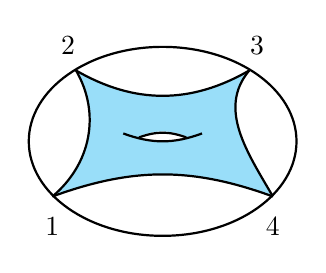
\begin{tikzpicture}[anchor=base,baseline]
	\node [coordinate] (BL) at (-1.4,-.7) {};
	\node [coordinate] (TL) at (-1.1, .9) {};
	\node [coordinate] (BR) at ( 1.4,-.7) {};
	\node [coordinate] (TR) at ( 1.1, .9) {};
	\node at (-1.4,-1.2) {$1$};
	\node at (-1.2, 1.1) [] {$2$};
	\node at ( 1.4,-1.2) [] {$4$};
	\node at ( 1.2, 1.1) [] {$3$};
    \draw [thick] (0,0) ellipse (1.7 and 1.2);
    \fill[cyan,fill opacity=0.4] (BR) to [out=160,in=20] (BL)
    to [out=40,in=300] (TL)
    to [out=330,in=210] (TR)
    to [out=230,in=120] cycle;
	\draw [thick] (BR) to [out=160,in=20] (BL);
	\draw [thick] (BL) to [out=40,in=300] (TL);
	\draw [thick] (TL) to [out=330,in=210] (TR);
	\draw [thick] (TR) to [out=230,in=120] (BR);
    \fill[white] (-.28,.07) to [out=20,in=160] (.28,.07)
    to [out=340,in=200] cycle;
	\draw [thick] (-.3,.05) to [out=20,in=160] (.3,.05);
	\draw [thick] (-.5,.1) to [out=340,in=200] (.5,.1);
\end{tikzpicture}} \,
\sim \sum\limits_{\cO_5, \cO_6} \int dy_{5,6}
\Disc_{23}
\diagramEnvelope{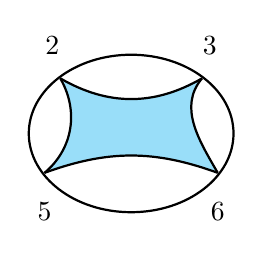
\begin{tikzpicture}[anchor=base,baseline]
	\node [coordinate] (BL) at (-1.1,-.5) {};
	\node [coordinate] (TL) at (-.9, .7) {};
	\node [coordinate] (BR) at ( 1.1,-.5) {};
	\node [coordinate] (TR) at ( .9, .7) {};
	\node at (-1.1,-1.1) {$5$};
	\node at (-1., 1.) [] {$2$};
	\node at ( 1.1,-1.1) [] {$6$};
	\node at ( 1., 1.) [] {$3$};
    \draw [thick] (0,0) ellipse (1.3 and 1.);
    \fill[cyan,fill opacity=0.4] (BR) to [out=160,in=20] (BL)
    to [out=40,in=300] (TL)
    to [out=330,in=210] (TR)
    to [out=230,in=120] cycle;
	\draw [thick] (BR) to [out=160,in=20] (BL);
	\draw [thick] (BL) to [out=40,in=300] (TL);
	\draw [thick] (TL) to [out=330,in=210] (TR);
	\draw [thick] (TR) to [out=230,in=120] (BR);
\end{tikzpicture}}
\Disc_{14}
\diagramEnvelope{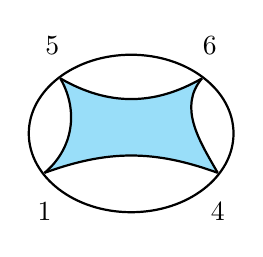
\begin{tikzpicture}[anchor=base,baseline]
	\node [coordinate] (BL) at (-1.1,-.5) {};
	\node [coordinate] (TL) at (-.9, .7) {};
	\node [coordinate] (BR) at ( 1.1,-.5) {};
	\node [coordinate] (TR) at ( .9, .7) {};
	\node at (-1.1,-1.1) {$1$};
	\node at (-1., 1.) [] {$\tl 5$};
	\node at ( 1.1,-1.1) [] {$4$};
	\node at ( 1., 1.) [] {$\tl 6$};
    \draw [thick] (0,0) ellipse (1.3 and 1.);
    \fill[cyan,fill opacity=0.4] (BR) to [out=160,in=20] (BL)
    to [out=40,in=300] (TL)
    to [out=330,in=210] (TR)
    to [out=230,in=120] cycle;
	\draw [thick] (BR) to [out=160,in=20] (BL);
	\draw [thick] (BL) to [out=40,in=300] (TL);
	\draw [thick] (TL) to [out=330,in=210] (TR);
	\draw [thick] (TR) to [out=230,in=120] (BR);
\end{tikzpicture}}
\end{equation*}
\caption{In the Regge limit the dDisc of the genus one closed string amplitude in AdS is given by the perturbative CFT optical theorem in terms of genus zero amplitudes.}
\label{fig:optical_theorem_string_pictures}	
\end{figure}
In the second part of the paper, we employ the perturbative CFT optical theorem in the context of the AdS/CFT correspondence \cite{Maldacena:1997re,Witten:1998qj,Gubser:1998bc}
to study high-energy scattering of strings in AdS, which is governed by the CFT Regge limit \cite{Cornalba:2006xk,Cornalba:2006xm}. This is illustrated in figure \ref{fig:optical_theorem_string_pictures}.
High-energy string scattering in flat space has been of interest for a long time, both in the fixed angle case \cite{Gross:1987kza,Gross:1987ar} and in the fixed momentum transfer Regge regime \cite{Amati:1987wq,Amati:1987uf,Amati:1988tn}. This second set of works studied the effects of the finite string size on the exponentiation of the phase shift (eikonalization) in the Regge limit. In particular, 
it was shown that the amplitudes indeed eikonalize provided we allow the phase shift to become an operator acting on the string Hilbert space, whose matrix elements account for the possibility of the external particles becoming intermediate excited string states, known as tidal excitations.
The phase shift $\de(s,b)$, which depends on the Mandelstam $s$ and on the impact parameter $b$, is 
obtained by Fourier transforming the amplitude with respect to momentum transfer 
in the directions transverse to the scattering plane. This gives a multiplicative optical theorem of the form
	\bea
		\Im \de_{\text{1-loop}}(s,b) 
		={}& \frac{1}{2} \sum\limits_{\substack{m_5,\rho_5,\e_5\\m_6,\rho_6,\e_6}}
		\de_\text{tree}^{3652}(s,-b)^* \,\de_\text{tree}^{1564}(s,b)\,,
	\eea{eq:impact_optical_theorem_flat}
where the sum is over all possible exchanged particles, characterized by their mass $m_i$ and Little group representation $\rho_i$,
and their polarization tensors $\epsilon_i$.
In \cite{Amati:1987uf} the one-loop amplitude for four-graviton scattering in type IIB string theory was presented in a particularly nice form, where the tidal excitations, which constitute a complicated sum in \eqref{eq:impact_optical_theorem_flat}, are packaged into a single explicit scalar function, the so-called vertex function.
 
To study the analogous process in AdS we derive an AdS/CFT analogue of \eqref{eq:impact_optical_theorem_flat} by transforming the correlators in the CFT optical theorem \eqref{eq:cft_optical_theorem_intro} to AdS impact parameter space \cite{Cornalba:2006xk,Cornalba:2006xm}. This gives the following multiplicative optical theorem for CFTs
\beq
-\Re \cB_{\text{1-loop}}(p,\bar{p})  \Big|_{\text{d.t.}} = \frac{1}{2}
\sum\limits_{\cO_5, \cO_6 \in s.t.}
\cB^{3652}_\text{tree}(-\pb,-p)^*  \, \cB^{1564}_\text{tree}(p,\pb)  \Big|_{[\cO_5 \cO_6]} \,.
\label{eq:gluing_stripped_intro}
\eeq
Here $\cB$ denotes the impact parameter transform of $A$. 
These transforms depend on two cross ratios $S$ and $L$, respectively interpreted as the square of the energy 
and as the impact parameter of the AdS scattering process,
that can be expressed in terms of two $d$-dimensional vectors $p$ and $\bar{p}$, as will be detailed below.
When ${\cO_5}$ or ${\cO_6}$ have spin,  $\cB$ has tensor structures that depend on
$p$ and $\bar{p}$.
Equations \eqref{eq:gluing_stripped_intro} and \eqref{eq:impact_optical_theorem_flat} are related through the flat space limit for the impact parameter representation, where the radius of AdS is sent to infinity and where $\cB(p,\bar{p})$ is mapped to $i \de(s,b)$.
In this way, each of the infinite number of tree-level correlators with spinning particles 5 and 6 that appear on the right hand side of \eqref{eq:gluing_stripped_intro} is partially fixed by the corresponding flat space phase shift. Moreover, we will be able to efficiently describe the summed result in terms of an AdS vertex function, 
which is in turn constrained by the one-loop flat space vertex function, as constructed for example for type IIB strings in  \cite{Amati:1987uf}.

For neutral scalar operators of dimension four in $d=4$, the four-point function considered here is dual to the scattering of four dilatons in the bulk of AdS$_5$. There are two expansion parameters that we need to consider, the loop order parameter $1/N^2$, and the t'Hooft coupling $\lambda$.
The large $\lambda$ limit is given by supergravity in AdS.
In this limit the tree-level four-point function is dominated by graviton exchange \cite{Cornalba:2006xk,Cornalba:2006xm} and beyond tree-level one can safely resum  the $1/N$ expansion by exponentiating the single graviton exchange \cite{Cornalba:2007zb,Brower:2007qh}.
For finite $\lambda$, string effects are included at tree-level via Pomeron exchange \cite{Brower:2006ea} and can
be described using conformal Regge theory \cite{Cornalba:2007fs,Costa:2012cb}. 
A very non-trivial question we address in this paper is the inclusion of string effects beyond tree-level.

To account for such effects in the Regge limit,  
the earlier works  \cite{Cornalba:2007fs,Cornalba:2008qf,Brower:2007xg}
conjectured the exponentiation of the tree-level Pomeron  phase shift, assuming stringy tidal excitations to be negligible \cite{Cornalba:2009ax}. 
More recently \cite{Meltzer:2019pyl}, the loop effects of Pomeron exchange were systematically taken into account from the CFT side in the AdS high-energy limit $S \gg \lambda \gg 1 $, with the crucial use of CFT unitarity to obtain higher-loop amplitudes from the lower-loop ones. This work also pointed out the suppression of tidal excitations in the supergravity limit $\lambda \gg 1$, in agreement with \cite{Cornalba:2007fs,Cornalba:2008qf,Brower:2007xg}. In the present work, we take finite $\lambda$ (or $\alpha'$) and include all tidal or stringy corrections. This is made possible because the perturbative CFT optical theorem is able to describe cuts involving spinning operators, so we can take into account
intermediate massive string excitations that are exchanged in the t-channel. 

This paper has the following structure. In section \ref{sec:glue}  we first motivate how \eqref{eq:general_contribution} for double-trace operators leads  to the perturbative CFT optical theorem \eqref{eq:cft_optical_theorem_intro} using the technique of ``conglomeration" \cite{Fitzpatrick:2011dm}, and then give a detailed derivation of \eqref{eq:cft_optical_theorem_intro} using tools from  harmonic analysis of the conformal group. Then in section \ref{sec:flat_space} 
we review some important ideas from flat space scattering, including impact parameter space, unitarity cuts and the vertex function, both to guide the AdS version and to serve as a target for the flat space limit. We subsequently move to the holographic case in section \ref{sec:ads}, where we transform the correlator to CFT impact parameter space to write a multiplicative optical theorem for phase shifts.
We use conformal Regge theory in the case of arbitrary spinning operators leading to the derivation of the AdS vertex function. In section \ref{sec:Appendix_tchannel} we recover the results for the one-loop correlator in the large $\lambda$ limit \cite{Meltzer:2019pyl} and also derive new t-channel constraints on CFT data at finite $\lambda$. We give the details of the flat space limit prescription in section \ref{sec:flat_space_limit}, and consider the specific four-dilaton amplitude of type IIB strings in section \ref{sec:IIB_AdS_flat}, constraining  several spinning tree-level correlators of the dual ${\cal N}=4$ SYM theory.
We conclude and briefly discuss some generalizations and applications of our work in section \ref{sec:conclusions}. Many technical details and additional considerations about spinning amplitudes are relegated to the appendices.



